\documentclass[14pt, aspectratio=169]{beamer}\usepackage[]{graphicx}\usepackage[]{color}
%% maxwidth is the original width if it is less than linewidth
%% otherwise use linewidth (to make sure the graphics do not exceed the margin)
\makeatletter
\def\maxwidth{ %
  \ifdim\Gin@nat@width>\linewidth
    \linewidth
  \else
    \Gin@nat@width
  \fi
}
\makeatother

\definecolor{fgcolor}{rgb}{0.345, 0.345, 0.345}
\newcommand{\hlnum}[1]{\textcolor[rgb]{0.686,0.059,0.569}{#1}}%
\newcommand{\hlstr}[1]{\textcolor[rgb]{0.192,0.494,0.8}{#1}}%
\newcommand{\hlcom}[1]{\textcolor[rgb]{0.678,0.584,0.686}{\textit{#1}}}%
\newcommand{\hlopt}[1]{\textcolor[rgb]{0,0,0}{#1}}%
\newcommand{\hlstd}[1]{\textcolor[rgb]{0.345,0.345,0.345}{#1}}%
\newcommand{\hlkwa}[1]{\textcolor[rgb]{0.161,0.373,0.58}{\textbf{#1}}}%
\newcommand{\hlkwb}[1]{\textcolor[rgb]{0.69,0.353,0.396}{#1}}%
\newcommand{\hlkwc}[1]{\textcolor[rgb]{0.333,0.667,0.333}{#1}}%
\newcommand{\hlkwd}[1]{\textcolor[rgb]{0.737,0.353,0.396}{\textbf{#1}}}%
\let\hlipl\hlkwb

\usepackage{framed}
\makeatletter
\newenvironment{kframe}{%
 \def\at@end@of@kframe{}%
 \ifinner\ifhmode%
  \def\at@end@of@kframe{\end{minipage}}%
  \begin{minipage}{\columnwidth}%
 \fi\fi%
 \def\FrameCommand##1{\hskip\@totalleftmargin \hskip-\fboxsep
 \colorbox{shadecolor}{##1}\hskip-\fboxsep
     % There is no \\@totalrightmargin, so:
     \hskip-\linewidth \hskip-\@totalleftmargin \hskip\columnwidth}%
 \MakeFramed {\advance\hsize-\width
   \@totalleftmargin\z@ \linewidth\hsize
   \@setminipage}}%
 {\par\unskip\endMakeFramed%
 \at@end@of@kframe}
\makeatother

\definecolor{shadecolor}{rgb}{.97, .97, .97}
\definecolor{messagecolor}{rgb}{0, 0, 0}
\definecolor{warningcolor}{rgb}{1, 0, 1}
\definecolor{errorcolor}{rgb}{1, 0, 0}
\newenvironment{knitrout}{}{} % an empty environment to be redefined in TeX

\usepackage{alltt}
\usetheme{Montpellier}
\usecolortheme{beaver}

\usepackage{amsmath, amssymb, ../../vimacros, hyperref, enumerate}
\usepackage{../../pdfpcnotes}
\usepackage[round]{natbib}

\usepackage{multicol}
\usepackage{physics}
\usepackage{xfrac}

\hypersetup{breaklinks=true, colorlinks=true, linkcolor=blue, citecolor=blue, urlcolor=blue}

\usepackage{tikz}
\usetikzlibrary{bayesnet}

\beamertemplatenavigationsymbolsempty

\title{Welcome and Introduction}
\date{}
\author{Philip Schulz \\
\url{https://vitutorial.github.io} \\
\url{https://github.com/vitutorial/VITutorial}}

\setbeamertemplate{footline}[frame number]

%% Load R packages


\IfFileExists{upquote.sty}{\usepackage{upquote}}{}
\begin{document}

\frame{\titlepage}

\begin{frame}{About me \ldots}

\begin{block}{Philip Schulz}
\begin{itemize}
\item Applied Scientist in the Clay team
\begin{itemize}
\item \texttt{clay-interest@amazon.com}
\end{itemize}
\item VI, Machine Translation, Bayesian Models
\end{itemize}
\end{block}
\end{frame}

\begin{frame}{What is a probabilistic model?}
A probabilistic model predicts \textbf{possible} outcomes of an experiment.
Most modern machine learning models are probabilistic.
\pause
\begin{block}{Maximum Likelihood}
\begin{equation*}
\underset{\theta}{\max}~p(x|\theta)
\end{equation*}
\end{block}
\end{frame}

\begin{frame}{Two Machine Learning Paradigms}
Supervised problems: \alert{``learn a distribution over observed data''}
\begin{itemize}
	\item \textcolor{gray}{sentences in natural language, images, videos, \ldots}
\end{itemize}

~

Unsupervised problems: \alert{``learn a distribution over observed and unobserved data''}
\begin{itemize}
	\item \textcolor{gray}{sentences in natural language + parse trees, images + bounding boxes \ldots}
\end{itemize}

\pnote{Q: LM supervised or unsupervised?} 

\end{frame}

\begin{frame}{What are the benefits of probabilistic models?}
Probabilistic models allow to incorporate assumptions through:
\begin{itemize}
\item the choice of distribution
\item the way that distribution uses side information
\item stipulate unobserved data
\end{itemize}
\pause
They return a distribution over outcomes.
\end{frame}

\begin{frame}{What are the benefits of probabilistic models?}
\begin{itemize}
\item Can generate data (generative models)
\pause
\item Allows to model unobserved data
\begin{itemize}
\item $ \intl{p(x|z,y)p(z|y)}{z} $ can be easier than $ p(x|y) $
\item Can reduce number of parameters
\item Provides explanation and can suggest improvements
\end{itemize}
\pause
\item Informative to decision makers
\begin{itemize}
\item Provides uncertainty estimates
\end{itemize}
\end{itemize}


\end{frame}

%\begin{frame}{What are the benefits of probabilistic models?}
%Probabilistic models can help by inferring \textbf{unseen} data. This also adds structure to the problem.
%\begin{block}{Latent Variables}
%Instead of
%\begin{equation*}
%\underset{\theta}{\max}~p(x|\theta)
%\end{equation*}
%try to account for latent data
%\begin{equation*}
%\underset{\theta}{\max}~\E[p(z|\theta)]{p(x|z,\theta)}
%\end{equation*}
%\end{block}
%\end{frame}

\begin{frame}{What are the benefits of probabilistic models?}
We can get uncertainty estimates.
\begin{block}{Example: Binary classifier}
\begin{equation*}
\sigma\left(x^{T}\theta\right)
\end{equation*}
gives \textbf{one} distribution over outcomes.
\end{block}
A decision maker wants to know \textbf{how much} he can trust the classifier!
\end{frame}

\begin{frame}{What are the benefits of probabilistic models?}
\begin{equation*}
\sigma\left(x^{T}M\theta\right) p(M)
\end{equation*}
where $ M $ is some matrix that modifies the classifier weights. \pause
This gives us many different distributions over outcomes!
\pause
\begin{block}{Rule of Thumb}
If the different distributions are similar, the classifier can be trusted. If they are dissimilar, further context information is needed.
\end{block}
\end{frame}

\begin{frame}{What are the benefits of probabilistic models?}
\begin{knitrout}
\definecolor{shadecolor}{rgb}{0.969, 0.969, 0.969}\color{fgcolor}

{\centering 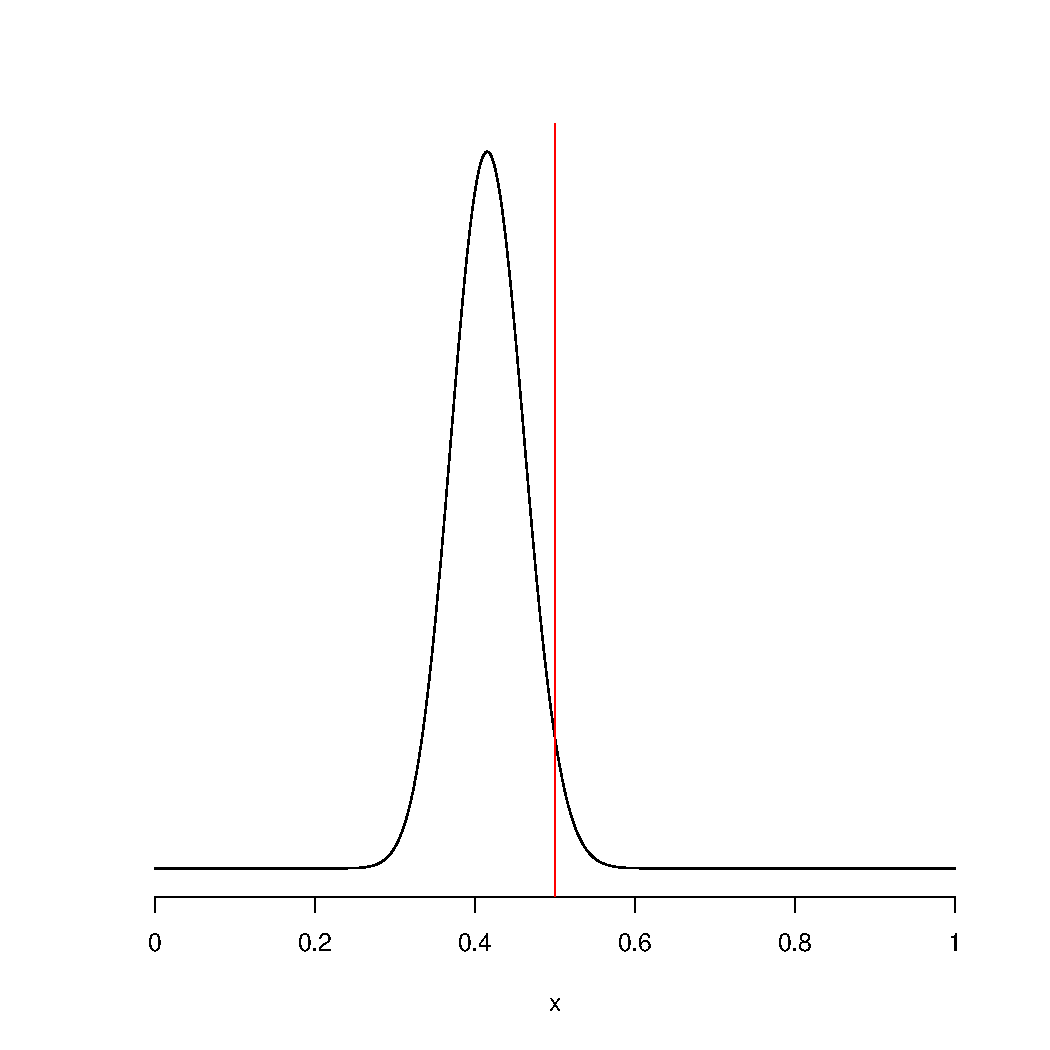
\includegraphics[width=\maxwidth,height=.95\textheight,keepaspectratio]{figures/beta_narrow-1} 

}



\end{knitrout}
\end{frame}

\begin{frame}{What are the benefits of probabilistic models?}
\begin{knitrout}
\definecolor{shadecolor}{rgb}{0.969, 0.969, 0.969}\color{fgcolor}

{\centering 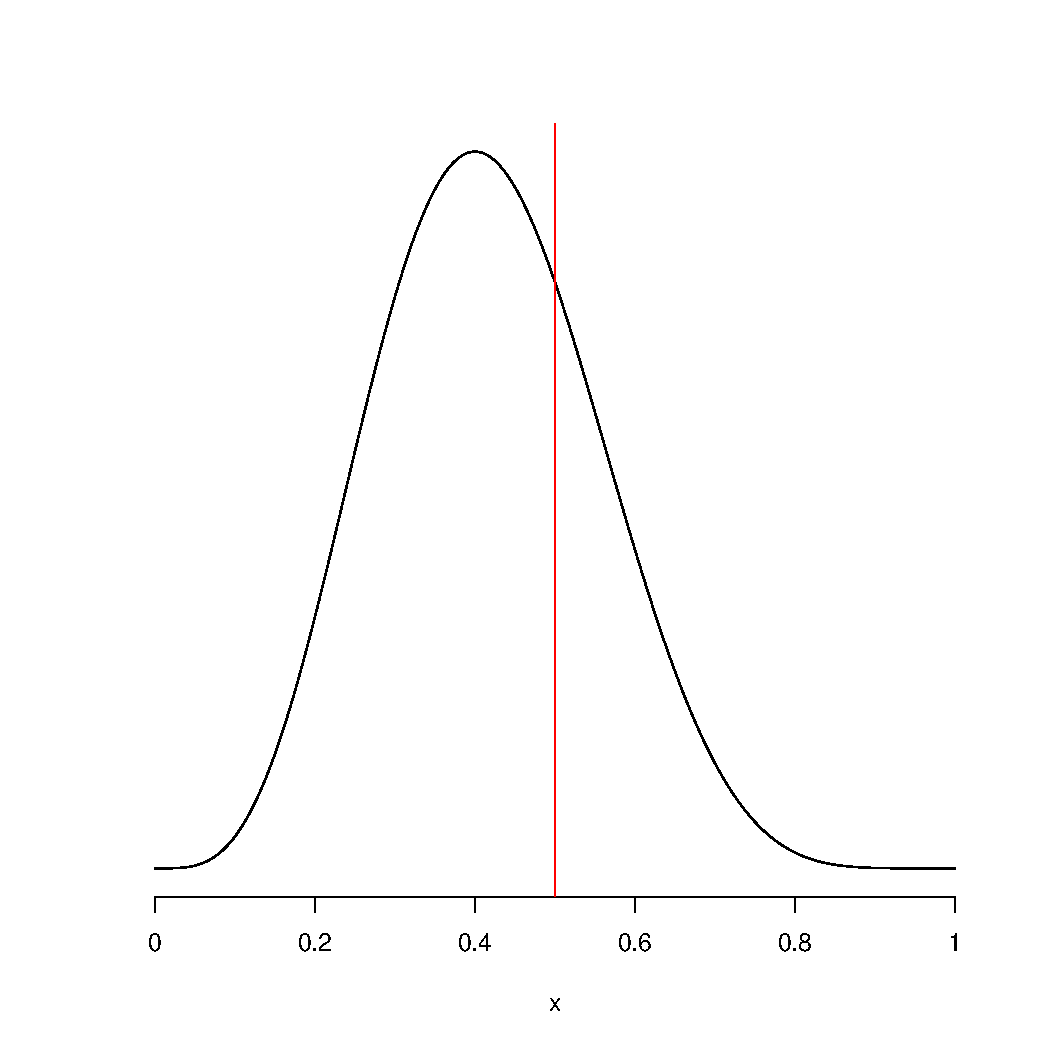
\includegraphics[width=\maxwidth,height=.95\textheight,keepaspectratio]{figures/beta_wide-1} 

}



\end{knitrout}
\end{frame}

\begin{frame}{Deep Generative Models}
Naturally, one would like to combine the advantages of probabilistic models and neural nets. So why not have a neural net with latent variables? \\
Short answer: backpropagation breaks!
\end{frame}

\begin{frame}{Deep Generative Models}
\begin{block}{Supervised MLE}
$ \underset{\phi}{\max}~p(x|\phi,y) \implies \underset{\theta}{\max}~p\left(x|\text{NN}_{\theta}(y)\right) $
\begin{itemize}
\item $ \phi = (\mu, \sigma) $, $ \phi = (\theta_{1}, \ldots, \theta_{K}) $, \ldots
\end{itemize}
\end{block}
\pause
\begin{block}{Unsupervised MLE}
$ \underset{\phi}{\max}~p(x|\phi,y, z)p(z|y, \phi) \implies \underset{\theta}{\max}~p\left(x|\text{NN}_{\theta}(z,y)\right) p\left(z|\text{NN}_{\theta}(y)\right) $
\begin{itemize}
\item $ \phi = (\mu_{x}, \sigma_{x}, \mu_{z}, \sigma_{z}) $, \ldots
\end{itemize}
\end{block}
\end{frame}

%\begin{frame}{Supervised Learning}
%\pnote{Q: Why computing the exact gradient is inconvenient?} 
%
%For large $\alert{N}$, we can use a \textbf{stochastic} gradient estimate 
%\begin{small}
%\begin{equation*}
%\begin{aligned}
%\grad_\theta \mathcal L(\theta, x^{(1:N)}) &=   \underbrace{\sum_{s=1}^{\alert{N}} \grad_\theta \log p(x^{(s)}|\theta)}_{\text{too many terms}} \\ \pause
%&=   \sum_{s=1}^{\alert{N}} \textcolor{blue}{\frac{1}{ N} } N \grad_\theta \log p(x^{(s)}|\theta) \\ \pause
%&= \sum_{s=1}^{\alert{N}}\textcolor{blue}{\mathcal U(s|\sfrac{1}{N})}  N \grad_\theta \log p(x^{(s)}|\theta) \\ \pause
%&= \mathbb E_{S\sim \mathcal U(\sfrac{1}{N})}\left[ N \grad_\theta  \log p(x^{(S)}|\theta)\right]
%\end{aligned}
%\end{equation*} 
%\end{small}
%\end{frame}
%
%\begin{frame}{Supervised Learning}
%
%\pnote{Q: Why should we like expected gradients?} 
%
%For large $\alert{N}$, we can use a \textbf{stochastic} gradient estimate 
%\begin{small}
%\begin{equation*}
%\begin{aligned}
%\grad_\theta \mathcal L(\theta,x^{(1:N)}) 
% &=  \mathbb E_{S\sim \mathcal U(\sfrac{1}{N})}\left[ N \grad_\theta  \log p(x^{(S)}|\theta)\right] \\ \pause
% &\overset{\text{MC}}{\approx} \frac{1}{M} \sum_{m=1}^M N  \grad_\theta \log p(x^{(s_i)}|\theta) ~~~S_i \sim \mathcal U(\sfrac{1}{N})
%\end{aligned}
%\end{equation*}
%\end{small}  \pause
%where $x^{(s_1:s_M)}$ is a random mini-batch of size $M$
%
%
%\end{frame}

\begin{frame}{Unsupervised Learning}
Exact gradient is intractable
\begin{small}
\begin{equation*}
\begin{aligned}
\grad_\theta \log p(x|\theta) \pause &= \grad_\theta \log \int p(x, z|\theta) \dd{z} \\ \pause
&= \underbrace{\frac{1}{\textcolor{blue}{\int p(x, z|\theta) \dd{z}}} \int \grad_\theta p(x,z|\theta) \dd{z}}_{\text{chain rule}} \\ \pause
&= \frac{1}{\textcolor{blue}{p(x|\theta)}} \int \underbrace{p(x,z|\theta) \grad_\theta \log p(x,z|\theta)}_{\text{log-identity for derivatives}} \dd{z} \\ \pause
&= \int \alert{p(z|x, \theta)} \grad_\theta \log p(x,z|\theta) \dd{z} \\ \pause
&= \mathbb E_{\alert{p(z|x, \theta)}} \left[ \grad_\theta \log p(x,Z|\theta) \right]
\end{aligned}
\end{equation*}
\end{small}
\end{frame}

\begin{frame}{Variational Inference}
Computing the posterior distribution $ p(z|x, \theta) $ is hard. In VI we will optimize an auxiliary distribution $ q(z|x, \lambda) $ to approximate the exact posterior.
\end{frame}

\begin{frame}{What are you getting out of this today?}

As we progress we will
\begin{itemize}
	\item develop a shared vocabulary to talk about generative models powered by NNs
	\item derive crucial results step by step
\end{itemize}

\pause

Goal
\begin{itemize}
	\item you should be able to navigate through fresh literature
	\item and start combining probabilistic models and NNs
\end{itemize}

\end{frame}

\end{document}
